%!TEX root = project.tex

\chapter*{About this project}
\paragraph{Abstract}
A brief description of what the project is, in about two-hundred and fifty words.

\paragraph{Authors}
Explain here who the authors are.



\chapter{Introduction}

\section{Outline}
The aim of this project is to develop a full stack weather application that use's machine learning to predict certain weather conditions. There are dozens of weather applications available today that give a wide variety of information on future weather. However, most of these applications depend solely on API data and very few integrate both API and machine learning data into one application.

\section{Background}
Millions of people around the world regularly acquire information from weather forecasts for a large number of reasons. The increased growth in accessibility to the internet has allowed for a more suitable way for people to retrieve this information, in recent years; weather applications have quickly gained in popularity.

The weather is always changing, and its conditions influence our daily lives, influencing what we choose to do and how we go about our day. Weather’s dynamic nature, however, means that factors such as temperature and precipitation are often constantly changing. It is for this reasons people want to know in detail what effects the forecast conditions will have so that they can plan. \cite{WeatherontheGo} With the ever changing weather there is a need for weather stations to provide accurate data to allow for more accurate forecasts.

The equipment used to collect weather data across Ireland varies depending on the four different types of weather stations, Manned Weather Stations which record meteorological elements on an hourly basis using a form, as seen in figure \ref{MetForm}, Automatic Weather Stations record meteorological elements on a minute-by-minute basis, Climatological Stations records data for climate analysis and meteorological research, Rainfall Stations record daily and monthly rainfall data due to Ireland having extremely distributed rainfall there are over five hundred of these stations \cite{MET}. There are many  

\begin{figure}[h]
\centering
\includegraphics[scale=0.4]{img/MannedWeatherStation.jpg}
\caption{Form used by meteorological observer at a manned station}
\label{MetForm}
\end{figure}
weather instruments used to gather data but since this paper is focusing on the prediction of Temperature and Rainfall values, I will only discuss the instruments relevant with the above.

Thermometers measure the high and low outdoor temperature in degrees Celsius or Fahrenheit. Today electronic maximum-minimum temperature sensor systems are used, see figure \ref{Thermometer} rather than back in the 1800s when they used liquid in glass thermometers.\cite{WeatherInstruments}

\begin{figure}[h]
\centering
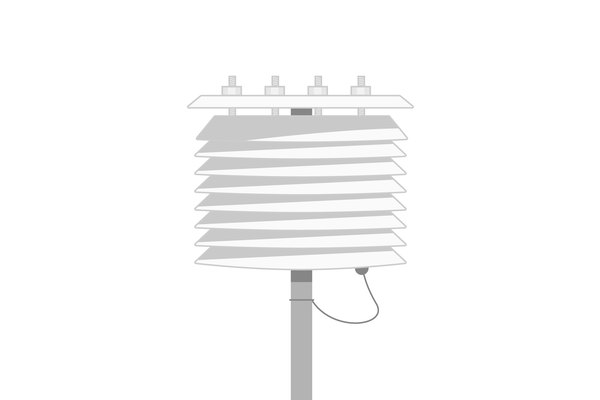
\includegraphics[scale=0.2]{img/MaxMinThermometer.jpg}
\caption{Electronic Thermometer used to collect temperature data.}
\label{Thermometer}
\end{figure}

Rain gauges measure the amount of rainfall. There are two types of rain gauges: The Storage Rain Gauge and The Tipping Bucket Rain Gauge see figure \ref{Gauge}. The latter is used more widely due to it being more automated and fewer hands on.\cite{RainGauge}

\begin{figure}[h]
\centering
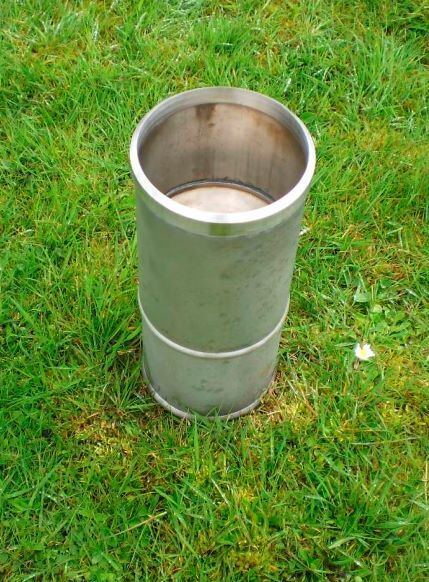
\includegraphics[scale=0.2]{img/storageRainGauge.jpg}
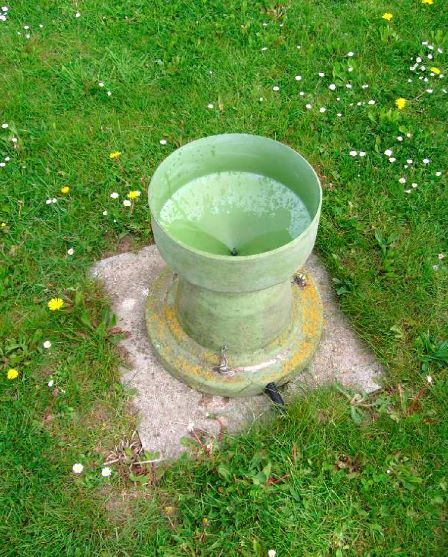
\includegraphics[scale=0.2]{img/tippingBucketGauge.jpg}
\caption{The Storage Rain Gauge and The Tipping Bucket Rain Gauge}
\label{Gauge}
\end{figure}

\section{WEB APPLICATION DEVELOPMENT}
A Web Application (WA) is a computer program that utilizes web browsers and web technology to perform tasks over the Internet. Web application development is the creation of application programs that reside on servers and are delivered to the users device over the Internet \cite{WebAppDef}.

WA's use a combination of server-side scripts (Django) to handle the storage and retrieval of data, and client-side scripts (React) to display that data to users \cite{WebApp}. Client-side refers to an application running on a web browser.Client-side programming typically utilizes HTML, CSS, JavaScript combined with a frontend framework such as React. Server-side programming powers the client-side programming and is used to create scripts that enables the web application to have various features. Server-side programming has many different coding languages such as Python, Ruby, Java \cite{WebAppDef}.

Data is exchanged over the network using HyperText Transfer Protocol (HTTP). An advantage of this approach is that the users do not depend on any specific operating system or hardware configuration. Hence, WA's are cross-platform software. They vary in functionality and design but are setup to serve the same purpose, which is to provide the user with features and accessibility to information.

The application developed would provide consistent weather forecast updates and will be a significant improvement compared with similar websites by allowing access to more premium features from anywhere any location. 

\section{HISTORY OF MACHINE LEARNING}
Machine Learning (ML) which is a sub-set of artificial intelligence where computers can self learn from data and information. ML algorithms automatically build a model of sample data also known as — "training data" — to make decisions without being specifically programmed to make those decisions \cite{MLAlgorithms}.

The first computer learning program was written by Arthur Samuel in 1952. He designed a program which was a game of checkers, the program used a minimax strategy to decide on the next move. After playing more games it studied which moves made up winning scenarios and incorporated these into the program. The minimax strategy later became known as the "Minimax Algorithm" \cite{MiniMax}.

Later that same decade in 1957, Frank Rosenblatt designed "The Perceptron" which was first neural network for computers. It was designed with efforts of Donald Hebb's model of brain cell interaction and Arthur Samuel's ML knowledge to simulate the thought process of the brain. In the years 1967 to the early 2000s there was were many developments in the ML area such as the "nearest neighbour" algorithm which allowed computers to use basic pattern recognition, the concept of Explanation Based Learning which a computer analyses data and creates a rule to discard unimportant data. ML shifted from knowledge-driven approach to data-driven approach, creating programs that could analyze large amounts of data and learn from the results \cite{MLAlgorithmsHistory}.

The late 2000s is when ML started to gain recognition outside of the computer world due to ML featuring in more widely used devices such as The Microsoft Kinect which allowed users to interact using gestures, Facial Recognition being used in mobile devices for security purposes and speech recognition which is done by a deep learning technique called Long Short-Term Memory (LSTM) is used in Apples Siri \cite{MLAlgorithmsHistory}.

Present day ML in responsible for some of the great advancements in technology, such as self-driving vehicles and talking robots. ML models have become increasingly more efficient in continuously learning from training data which in turn makes them more accurate with increased data to learn from. Ml models can be used for a variety of reasons from predicting the weather to predicting stock prices.
\newpage
\section{SCOPE OF THE PROJECT}
\begin{enumerate}
\item User friendly web application.
\item Fully functional weather predictions.
\item Consistent forecasts.
\item Login and Register system.
\item About page providing information on application.
\item Visually pleasing design.
\item Similar features to competitor applications.
\end{enumerate}

\chapter{Context}
\section{Project Objectives}
In this section I will outline the key objectives for this section.
\begin{itemize}
    \item To provide an aesthetically pleasing UI.
    \item To provide a reliable weather application.
    \item To provide REST API to weather forecasts.
    \item To provide a scalable application.
    \item To provide user security with storage of personal information.
    \item To provide low load times when retrieving information.
\end{itemize}

\section{Weather Application}
A weather application is increasingly important in today's modern world, with more easier access to online resources and access from nearly any location with a mobile phone signal it has led to a significant rise in numbers using web applications. Gone are the days of waiting for specific times in the day to tune in for the daily/weekly weather reports on the radio/TV. The use of weather applications that are supported on any device with a browser has led to a revolution in the way we get the latest weather. In this chapter I will discuss the advantages, disadvantages and overall impact of weather applications.

\section{Advantages of Weather Applications}
This section I will discuss the advantages of weather applications.

\subsection{Reliability}
There are many advantages to weather applications which I will discuss in this section, the most noteworthy of those is reliability. Taking into consideration the advancements in weather data collection in recent years has led to more widely available weather information, which in-turn provides weather applications with more reliable forecasts. Users of these applications can now know what the weather will be like within the next week, a weather forecast can give you a really good idea of what to expect. A seven-day forecast can accurately predict the weather about 80 percent of the time and a five-day forecast can accurately predict the weather approximately 90 percent of the time \cite{weatherReliability}. 

\subsection{Competitors}

The rise in various weather applications over the years means that each application is trying to add new features to stand out from the crowd. The customer benefits from this competitive nature within these businesses allowing them to have more choice in which application they use. 
\subsection{Convenience}
Frequent users of weather application now only have to open an application on their smart device to gain access to tonnes of weather information. The user can now plan there day/week in advance at any moment rather than having to wait for a certain time in the day when the weather report would be on a radio or TV. The benefit of this convenience is that the user gains more information at a touch of button and they save time looking for weather forecasts when its all in the one area.

\section{Disadvantages of Weather Applications}
This section I will discuss the disadvantages of weather applications.

\subsection{Inaccurate weather predictions}

Weather predictions are never 100\% and it is almost impossible to predict the future with certainty. Even if you have a great process in place and forecasting experts on your payroll, your forecasts will never be spot on. Some applications will have high level of volatility depending on which weather data provider they are using. The main drawback of forecasts are that they are almost always inaccurate - which leads to a dissatisfied customers.

\subsection{Security}

Storing details in a digital environment is a lot less secure than storing those same details in non digital environment. The reason for this is due to that data being stored on a server that is vulnerable to attacks such as SQL Injection - Occurs when a perpetrator uses malicious SQL code to manipulate a backend database so it reveals information. Consequences include the unauthorized viewing of lists, deletion of tables and unauthorized administrative access \cite{sqlInjection}. Gaining access to such a database on a weather application may hold users personal details, card details and address details.

\subsection{Internet Reliance}

An internet connection is a must with web application for it to load any data. There will be a lack of updated information if internet connectivity is lost during browsing. Web applications cannot run without internet which makes them redundant in areas with little to no internet. 

\section{The Overall Effect of Weather Applications}

The overall effect of weather applications has had a resounding impact on the way customers plan ahead. The reliability and convenience of everyday weather applications to the mass population of the world has led to more advantages than disadvantages in my personal opinion.
\newpage
\section{Outline of each chapter}
Below I will outline the chapters that my Dissertation is broken up into and give a brief outline of each one.

\subsection{Introduction}
In Chapter 1, I will give an outline of the overall project and then proceed to discuss the background of weather. I will then discuss web application development and the history of machine learning to give the reader an understanding of the project.

\subsection{Context}
In Chapter 2, I will discuss the context of my project and how weather applications have changed how we view the weather. I will research the advantages and disadvantages of weather applications for users.

\subsection{Methodology}
In Chapter 3, I will discuss the methodology I followed and how it affected my project and productivity. I will also discuss how I planned to complete the project and discuss the methodologies I utilized in the process. I will discuss why I chose these methodologies and give the reader an insight into how this application was developed. 

\subsection{Technology Review}
In Chapter 4, I will discuss the technical aspects of this project and discuss how each technology impacted the development cycle of this project. I will also discuss why each technology was implemented over other available technologies. I will discuss the three main technologies chosen for this project in detail and how I utilized each of them to create a Full Stack Weather Application. 

\subsection{System Design}
In Chapter 5, I will explain the architecture and design of the project. I will use graphs, diagrams and screen shots to help explain the rationale of how the application is designed and how it will operate when deployed. I will discuss various main functions in the code to give an overview of how the main features of the application work.

\subsection{System Evaluation}
In Chapter 6, I will test the software and evaluate whether it is robust and meets all the objectives I have specified. I will highlight any limitations in the approach used and the technologies used.

\subsection{Conclusion}
In Chapter 7, I will outline what I have learned from this project and highlight any findings from the system evaluation chapter. I will discuss the impact the project had on my skills as software developer and how working remotely during a global pandemic impacted the development stage of the project. I will also summarise the what I would do differently if I was to do this project again.

\section{Github Structure}

The \href{https://github.com/MarkReillyGMIT/AppliedProject}{Github} resource URL can be found by clicking \href{https://github.com/MarkReillyGMIT/AppliedProject}{Here}. The git repository contains four folders: Dissertation, ReadMeFiles, backend and front-end. The Dissertation folder contains all files related to the development of the dissertation document. The ReadMeFiles folder contains all images that will be displayed on the README. The backend folder contains all the related code for the Django backend and neural network computation. The front-end folder contains all the related code for the React front-end. There is a requirements.txt file that has all the required libraries necessary for the project to run. The README.md file will contain a brief description of the project and how to run the project. The gitignore file is a text file that tells Git which files or folders to ignore in a project. 


\chapter{Methodology}

\section{Overview of Methodology}

In this project I took an agile approach to development using the Agile Methodology. I used sprints to manage my work during the development life-cycle.

\section{Agile}
In this section I will discuss the Agile Methodology which was utilized in the development process of this application.

\subsection{What is Agile?}
AGILE methodology is a practice that promotes continuous iteration of development and testing throughout the software development life cycle of the project. In the Agile model, both development and testing activities are concurrent, unlike the Waterfall model\cite{Agile}. Agile is a term used to describe software development approaches that employ continual planning, learning, improvement, team collaboration, evolutionary development, and early delivery. It encourages flexible responses to change \cite{Agile}. There are many different agile methodologies to chose from such as Kanban, Scrum, Extreme Programming (XP), Crystal, Dynamic Systems Development Method (DSDM). For the purpose of this project I will be using Scrum. 

\begin{figure}[h]
\centering
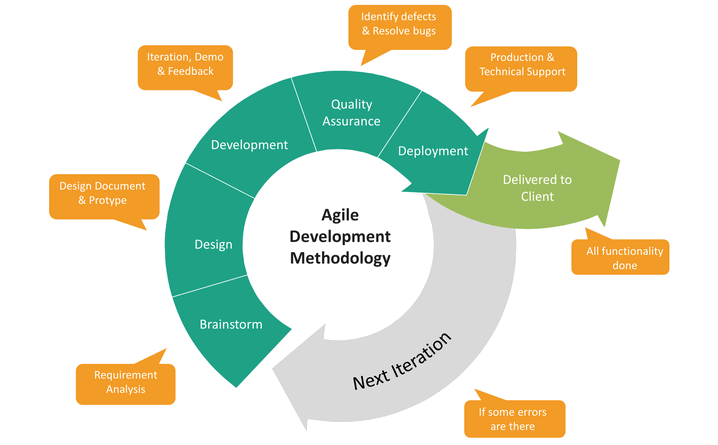
\includegraphics[scale=0.4]{img/agile-development-chart.png}
\caption{Agile Development Lifecycle}
\label{Agile}
\end{figure}


\newpage

\section{What is Scrum?}
SCRUM is an agile development method which concentrates specifically on how to manage tasks within a team-based development environment. Basically, Scrum is derived from activity that occurs during a rugby match \cite{Agile}. Since SCRUM is mainly used for team projects I had to adapt it to suit my needs. It consists of three roles which are as follows:

\begin{itemize}
    \item Scrum Master - responsible for setting up the sprint meetings and removing challenges to progress \cite{Agile}.
    \item Product Owner -  creates the product backlog and is responsible for the delivery of the product. Sharing the vision for the product with the team \cite{Agile}.
    \item Scrum Team - manages its own work and organizes its work to finish the sprint of cycle \cite{Agile}.
\end{itemize}

\begin{figure}[h]
\centering
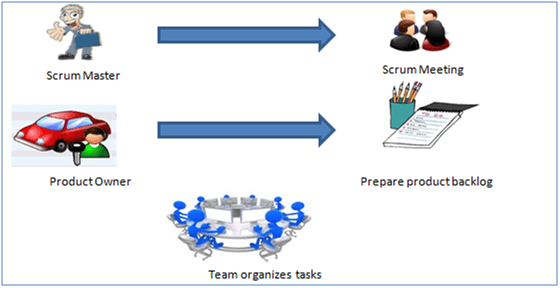
\includegraphics[scale=0.4]{img/scrum.png}
\caption{Scrum Development}
\label{Scrum}
\end{figure}

\subsection{Adapting Scrum}
In this section I will discuss how I adapted the scrum methodology into my individual project. 

During the project I dedicated time to planning the project weeks in advance. Using a Gantt Chart to plan and keep track of weekly tasks and milestones. The Gantt chart software that I used was on \href{https://app.clickup.com}{Clickup} which was provided for free. It allowed for the adding of tasks and milestones which then could be marked as "Open", "Closed", "Completed". There were also email notifications available that provided an update on tasks that were soon to be overdue. There was a lack of free Gantt Chart software available online which made it difficult and time consuming to find a good standard free version. See Figure \ref{Gantt}.

\begin{figure}[h]
\centering
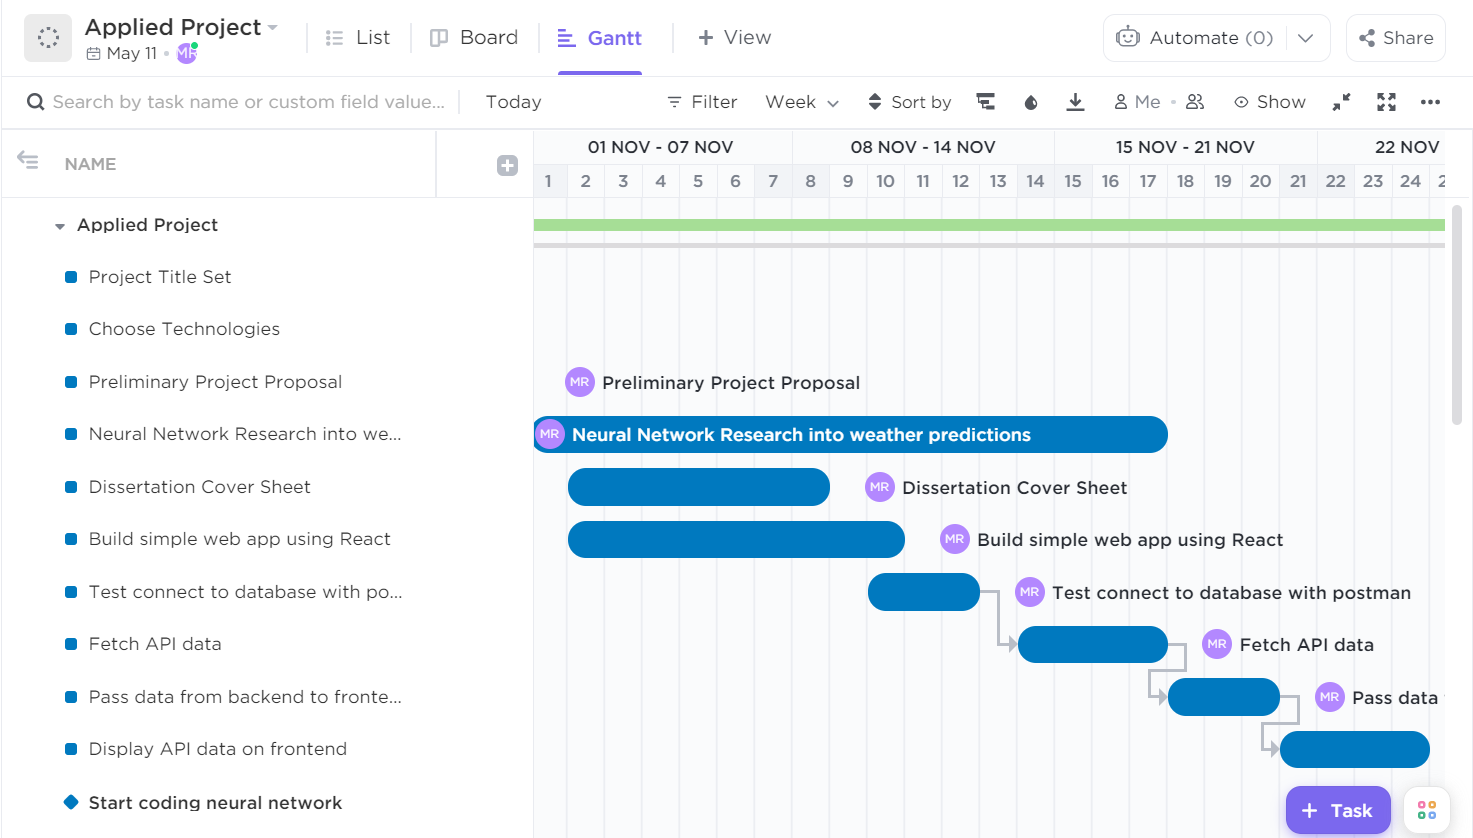
\includegraphics[scale=0.4]{img/GanttChart.PNG}
\caption{Gantt Chart}
\label{Gantt}
\end{figure}

\subsection{Planning Sprints}

I planned my sprints using the tasks on the gantt chart, each task was added with a certain amount of time depending on the difficulty of the task. Setting reasonable and attainable goals for each week. See Figure \ref{Gantt} to view the variable time lengths that were given to each task.

\subsection{Conduct Weekly Scrums}

I scheduled a time each week to review my previous weeks work to identify any successes and pitfalls \cite{Scrum}. I had to then act as the scrum master to find solutions to any problems I may have encountered that week. Referring to my Gantt chart for a visual idea of where I could find the time to fix the problems encountered.

\subsection{Review your sprint}
At the end of the sprint I would consider the downsides and upsides of the process. Taking into consideration the how closely the results align with the overall vision for the project \cite{Scrum}. 

\section{Test Driven Development}
In this section I will discuss Test Driven Development (TDD), what it is and how I incorporated it into the development process.

\subsection{What is Test Driven Development}
TDD is software development approach in which test cases are developed to specify and validate what the code will do. In simple terms, test cases for each functionality are created and tested first and if the test fails then the new code is written in order to pass the test and making code simple and bug-free \cite{TDD}. See Figure \ref{TDD}.

\begin{figure}[h]
\centering
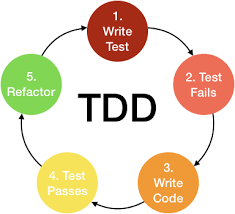
\includegraphics[scale=0.5]{img/TDD.png}
\caption{Test Driven Development Cycle}
\label{TDD}
\end{figure}

\subsection{How I incorporated TDD into the project}
I applied TDD into the project by writing tests into various parts of the code as I was in the development phase. I wrote print out statements to the command line for the backend to analyse the values that were being sent. For the front-end, I wrote tests that could be viewed using the inspect element to analyse the correct data that was being displayed on the web application. I continued to write enough code to make the test pass and then refactored it, repeating this process for each test. 

\section{Git Version Control}
In this section I will discuss version control and how I managed to develop the project by using Github and Git. I used \href{https://github.com/MarkReillyGMIT/AppliedProject}{Github} to manage all the code and files for the project while using Git to commit any new/update code to the Github repository. Using Github had many beneficial factors such as file management, project management tools and online file storage. 

In the project section on Github, I utilized the Kanban board which helped with managing any issues I was facing, and keeping track of each issue. Github also allows for multiple branches to be created which can be helpful for team projects but in this individual project I decided to only use the Master branch as I was the only person committing to this project.

Git version control allowed for the tracking of files and any changes made to each file. This really helped when needing to revert back to a previous working version of the project. 

\section{Time Management}
In this section I will discuss how I manage my time during the development phase of the project and the issues I faced throughout.

\subsection{Management of Several Projects}
I was able to manage multiple projects at time by using the Gantt chart to set out my weekly task and assigning different days to various different modules. The tasks sometimes became tough to complete on time as the workload of other modules was heavy at certain times of the year. 

\subsection{Issues Faced}
I faced many issues throughout the project as the workload was immense. Here list of the top issues faced:

\begin{itemize}
    \item Difficulty in finding a quite work environment due to college being closed.
    \item Standard of projects were dropped due to heavy workload.
    \item Slow internet due to location.
    \item Covid-19 illness.
    \item Procrastination. 
\end{itemize}
\newpage


\chapter{Technology Review}
\section{Overview}
In this chapter I will discuss the technologies used in this project at conceptual level. I will explain why I used these technologies, how they were implemented and utilized to allow for a fully functional weather application. I will also review each technology utilized and show how each technology gave a different functionality in reaching the end vision of the project. 

\section{ReactJS}
In this section I will discuss what ReactJS is and the features it provides.

\subsection{About ReactJS}
ReactJS is JavaScript library which is deployed to develop reusable user interface (UI) components. React basically enables development of large and complex web based applications or mobile applications which can change its data without subsequent page refreshes. React abstracts the Document Object Model (DOM), offering a simple, performing and robust application development experience \cite{aggarwal2018modern}. React is only concerned with state management and rendering that state to the DOM. Using React usually requires additional libraries for other functionality such as routing.


\subsection{Features of ReactJS}

\begin{figure}[h]
\centering

\includegraphics[scale=0.3]{img/ReactJS.png}
\caption{ReactJS}
\label{React}
\end{figure}

\section{Django}
\subsection{About Django}

\section{Database}
\subsection{Postgres}

\section{Architecture}

\section{APIs}

\section{Libaries}

\section{Languages}

\section{Styles}

\section{Cloud}

\section{Documentation}
\begin{itemize}
\item Describe each of the technologies you used at a conceptual level. Standards, Database Model (e.g. MongoDB, CouchDB), XMl, WSDL, JSON, JAXP.
\item Use references (IEEE format, e.g. [1]), Books, Papers, URLs (timestamp) – sources should be authoritative. 
\end{itemize}

\section{XML}
Here's some nicely formatted XML:
\begin{minted}{xml}
<this>
  <looks lookswhat="good">
    Good
  </looks>
</this>
\end{minted}

\chapter{System Design}
As many pages as needed.
\begin{itemize}
\item Architecture, UML etc. An overview of the different components of the system. Diagrams etc… Screen shots etc.
\end{itemize}

\begin{table}[h]
  \centering
  \begin{tabular}{x{2cm}p{3cm}}
    \toprule \\
    Column 1 & Column 2 \\
    \midrule \\
    Rows 2.1 & Row 2.2 \\
    \bottomrule
  \end{tabular}
  \caption{A table.}
  \label{table:mytable}
\end{table}

\chapter{System Evaluation}
As many pages as needed.
\begin{itemize}
\item Prove that your software is robust. How? Testing etc. 
\item Use performance benchmarks (space and time) if algorithmic.
\item Measure the outcomes / outputs of your system / software against the objectives from the Introduction.
\item Highlight any limitations or opportuni-ties in your approach or technologies used.
\end{itemize}

\chapter{Conclusion}
About three pages.

\begin{itemize}
\item Briefly summarise your context and ob-jectives (a few lines).
\item Highlight your findings from the evalua-tion section / chapter and any opportuni-ties identified.
\end{itemize}

